\section{Strømforsyning Design} \label{sec:Stroemforsyning_Design}

Som nævnt i systemarkitekturen forsyner strømforsyningen øvrig HW i systemet, undtagen selve varmelegemet og DevKit8000, der forsynes med 230V AC, og sensorerne, der forsynes med VEE (3.3V DC) fra PSoC Master.

Strømforsyningen forsynes med 12V DC max. 3A fra en laboratorieforsyning jf. Signalbeskrivelser på Tabel \ref{tbl:signalbeskriv} på side \pageref{tbl:signalbeskriv}. 
Alternativt kan anvendes en 12V transformer, der kobles til 230V AC. 

Strømforsyningen skal have 12V DC udgange til motor og blæsere, USB udgange med VDD til PSoC4 Pioneer Kits og en VDD udgang til USB strømspareskinnen.

\begin{figure}[h]
\centering 
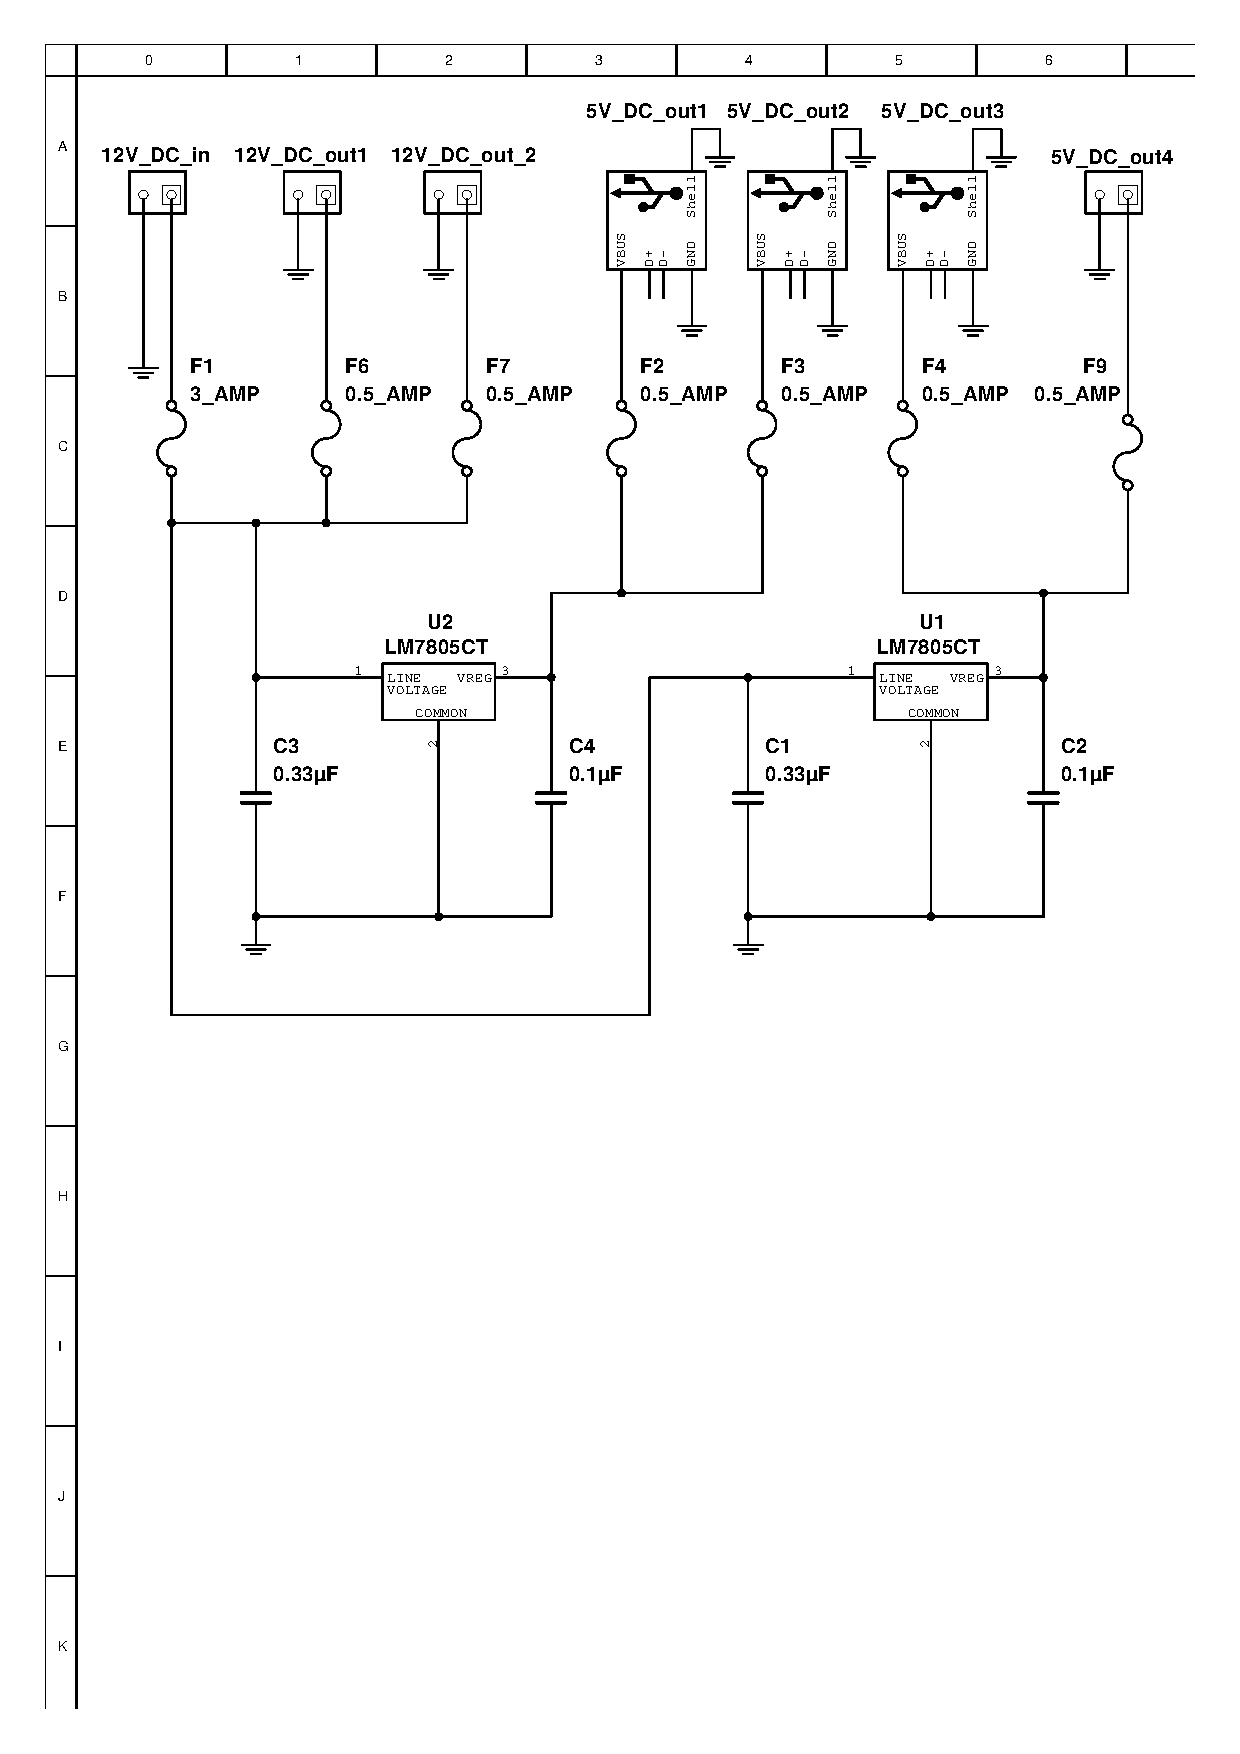
\includegraphics[width={\textwidth}, trim=50 350 30 40, clip=true] {../fig/multisim_stroemforsyning.pdf}
\caption{Diagram for blokken Strømforsyning}
\label{fig:multisim_stroemforsyning}
\end{figure}

Figur \ref{fig:multisim_stroemforsyning} viser Multisim diagram for designet af blokken Stroemforsyning. 
De enkelte komponenter og overvejelser herom gennemgås nedfor. 

\clearpage

12V DC in (VCC) trækker som sagt max. 3A, derfor monteres denne med en sikring på denne størrelse. 

12V DC out1 udgangen til motor trækker max. 500 mA jf. databladet \cite{lib:UHD2_DS} side 38, derfor monteres den med en sikring på 500 mA. 

De fire blæsere trækker hver især max. 140 mA ved fuld styrke jf. påtrykt værdi på selve blæserne. 
Implementeringen af koden i blokken Aktuator er lavet således, at blæserne maximalt kommer til at køre med en dutycycle på 50\%. 
Derfor monteres ligeledes en sikring på 500 mA til de fire blæsere. 

Ved en praktisk undersøgelse af USB skinnen konstateredes det, at USB indgangen trækker ca. 400 mA, når relæet er slået til, derfor monteres der også en 500 mA sikring på denne udgang. 

Der anvendes to spændingregulatorer LM7805, som begrænser 12V DC til 5V DC. 
De kan hver især levere 1A, derfor anvendes to stk. 
De monteres med afkoblinger til stel på ben 1 og 3 jf. standardapplikationen på side 1 i databladet \cite{lib:LM7805_DS}.

\clearpage

